\providecommand{\main}{../..}
\documentclass[../../main.tex]{subfiles}
\begin{document}

\subsection{Gaussian Integrals}
\lesson{3}{12/3/20}
In Statistical Mechanics, many integrals involve \textbf{gaussian} functions. 

These can be computed analytically in some quite general cases, as we now show, starting from the simplest case:
\begin{align}\label{eqn:gauss-int}
    I(b) \equiv \int_{\mathbb{R}} \dd{x} e^{-ax^2 + bx} = \sqrt{\frac{\pi}{a} } \exp\left(\frac{b^2}{4a} \right) \qquad a \in \mathbb{R}^+, \> b \in \mathbb{C}
\end{align}

\textbf{Proof}. When $b \in \mathbb{R}$, we can just \textit{complete the square} in the exponential argument:
\begin{align*}
    -ax^2 + bx = -a\left(x-\frac{b}{2a} \right)^2 + \frac{b^2}{4a} 
\end{align*}  
So that the integral becomes:
\begin{align*}
    I(b) &= \int_{\mathbb{R}} \dd{x} \exp\Bigg[-\underbrace{a\left(x-\frac{b}{2a} \right)^2 }_{y^2}+ \frac{b^2}{4a} \Bigg]
\shortintertext{We then \textit{extract} the constant term from the integral, and change variables:}
y &= \left(x - \frac{b}{2a} \right) \sqrt{a}
\shortintertext{So that $I(b)$ reduces to computing the integral of a standard gaussian:}
I(b) &= \frac{1}{\sqrt{a}} \exp\left(\frac{b^2}{4a} \right)  \underbrace{\int_{\mathbb{R}} \dd{y} e^{-y^2} }_{\sqrt{\pi}} = \sqrt{\frac{\pi}{a} } \exp\left(\frac{b^2}{4a} \right)
\end{align*}

In the case of $b = i \alpha$ (pure imaginary) we have:
\begin{align*}
    I(i \alpha) = \varphi_0(\alpha)
\end{align*}
where $\varphi_0$ is the characteristic function for the gaussian (with $a=1/(2\sigma^2) \Rightarrow \sigma = (2a)^{-1/2}$) already computed in example \ref{exa:char-gauss} at pag. \pageref{exa:char-gauss}, which confirms the result (\ref{eqn:gauss-int}). %Ref. will appear when compilating the entire document

\begin{exo}[General case]
    Prove formula (\ref{eqn:gauss-int}) in the most general case, where $b = \beta + i \alpha$. 

    \medskip

    \textit{Hint: translate the integration path in the complex plane, close it with the real line and apply the Cauchy Integral theorem.} 
\end{exo}

It is useful to generalize (\ref{eqn:gauss-int}) to the multidimensional case.

Let $\bm{x} \in \mathbb{R}^d$ and $A$ a $d\times d$ \textbf{symmetric} and \textbf{positive definite} matrix, i.e. such that:
\begin{align}\label{eqn:pos-def}
    \bm{x}^T A \bm{x} \equiv \sum_{i,j=1}^d x_i A_{ij} x_j > 0 \qquad \forall \bm{x} \neq \bm{0}
\end{align}  
The multi-dimensional Gaussian integral is defined as:
\begin{align*}
    I(A) \equiv \int_{\mathbb{R}^d} \dd[d]{\bm{x}} e^{-\bm{x}^T A \bm{x}}
\end{align*}
To solve it, the idea is to \textit{decouple} all the $n$ components, so that the integral becomes the product of $n$ gaussian integrals of the type (\ref{eqn:gauss-int}).

\medskip

This is done by using the spectral decomposition of $A$. As it is symmetric, it has $d$ eigenvectors $\bm{v_{\cdot\alpha}} = (v_{1\alpha}, \dots, v_{d \alpha})^T$ of eigenvalue $\lambda_\alpha$ (with $\alpha =1, \dots, d$) that form an orthonormal basis of $\mathbb{R}^d$ (spectral theorem):
\begin{align*}
    \bm{v}_\alpha^T \bm{v_\beta} = \delta_{\alpha \beta}
\end{align*}
If we then use the definition of eigenvector:
\begin{align*}
    A \bm{v_\alpha} = \lambda_\alpha \bm{v_\alpha}
\end{align*}
we arrive to:
\begin{align}
    \bm{v_\beta}^T A \bm{v_\alpha} = \lambda_\alpha \delta_{\alpha \beta} \label{eqn:on-decomp1}
\end{align}
Let $V$ be the matrix with the orthonormal eigenvectors of $A$ as columns: $V=(v_{\alpha \beta})_{\alpha, \beta=i,\dots, d}$. Then (\ref{eqn:on-decomp1}) can be put in matrix form:
\begin{align}\label{eqn:decomp2}
    V^T A V = \Lambda \underset{(a)}{\Rightarrow}  A =V \Lambda V^T
\end{align}
where $\Lambda = \operatorname{diag}(\{\lambda_\alpha\}_{\alpha=1,\dots,d}) = (\delta_{\alpha \beta} \lambda_\alpha)_{\alpha \beta=1, \dots, d}$, and in (a)
we used the fact that $V$ is an orthogonal matrix (as its columns are orthogonal to each other), and so $V^{-1} = V^T$. Equation (\ref{eqn:decomp2}) gives the \textbf{spectral decomposition}  of $A$.

\medskip

Substituting in the integral we get:
\begin{align*}
    I(A) = \int_{\mathbb{R}^d} \dd[d]{\bm{x}} e^{-\bm{x}^T A \bm{x}} = \int_{\mathbb{R}^d} \dd[d]{\bm{x}} \exp(-\bm{x}^T V \Lambda V^T \bm{x})
\end{align*}
Then we change variables $\bm{y} = V^T \bm{x} \Leftrightarrow \bm{x} = V \bm{y}$. The determinant of the jacobian is unitary, because $V$ is orthogonal. In fact, starting from $V^T V = \mathbb{I}$, we have:
\begin{align}\nonumber
   1 = \operatorname{det} \mathbb{I} = \operatorname{det}(V^T V) \underset{(a)}{=}  (\operatorname{det}V^T) (\operatorname{det}V) \underset{(b)}{=} (\operatorname{det} V) (\operatorname{det} V) = (\operatorname{det} V)^2\\
   \Rightarrow |\operatorname{det} V|=1 \span \label{eqn:unitary-det}
\end{align}
where in (a) we applied Binet's formula, and in (b) $\operatorname{det} V^T = \operatorname{det} V$.  

\medskip

So we arrive to:
\begin{align*}
    I(A) = \int_{\mathbb{R}^d} \dd[d]{\bm{y}} e^{-\bm{y}^T \Lambda \bm{y}} = \prod_{\alpha=1}^d \int_{\mathbb{R}} \dd{y_\alpha} e^{-y_\alpha^2 \lambda_\alpha} \underset{(a)}{=}  \prod_{\alpha=1}^d \sqrt{\frac{\pi}{\lambda_\alpha} }
\end{align*}
where in (a) we use (\ref{eqn:gauss-int}), as all components are now decoupled. 
To use (\ref{eqn:gauss-int}) we need all $\lambda_\alpha$ to be positive - which is indeed true, because the matrix $A$ is positive definite: 
\begin{align*}
    0 \underset{(\ref{eqn:pos-def})}{<}  \bm{v_\alpha}^T A \bm{v_\alpha} = \lambda_\alpha \bm{v_\alpha}^T \bm{v_\alpha} = \lambda_a \norm{\bm{v_\alpha}}^2 \Leftrightarrow \lambda_\alpha > 0
\end{align*}

Finally, note that:
\begin{align*}
    \operatorname{det}(A) \underset{(\ref{eqn:decomp2})}{=}
    \operatorname{det}(V \Lambda V^T) = 
    \textcolor{Red}{\cancel{\operatorname{det}(V^T)}} \operatorname{det}(\Lambda) \textcolor{Red}{\cancel{\operatorname{det}(V)}} \underset{(\ref{eqn:unitary-det})}{=}   \operatorname{det}\Lambda = \prod_{\alpha=1}^d \lambda_\alpha 
\end{align*}
And so we can rewrite:
\begin{align}\label{eqn:mult-gaussian}
    I(A) = \int_{\mathbb{R}^d} \dd[d]{\bm{x}} e^{-\bm{x}^T A \bm{x}} = \prod_{\alpha=1}^d \sqrt{\frac{\pi}{\lambda_\alpha}} = \pi^{d/2} (\operatorname{det}A )^{-1/2}
\end{align}

\begin{exo}[Generalization]
    Prove that:
    \begin{align}\label{eqn:generalized-gauss-int}
        I(A,\bm{b}) \equiv \int_{\mathbb{R}^d} \dd[d]{\bm{x}} e^{-\bm{x}^T A \bm{x} + \bm{b}^T \bm{x}} = \pi^{d/2} (\operatorname{det}A)^{-1/2} \exp\left(\frac{1}{4} \bm{b}^T A^{-1} \bm{b} \right)
    \end{align}
    where $A$ is a \textbf{symmetric}, \textbf{positive definite} $d\times d$ real matrix, and $\bm{b} \in \mathbb{C}^d$.  
\end{exo}

\subsection{Saddle Point approximation}
Let $f(\bm{x})$ be a function with a single minimum at $\bm{x_0}$ and such that:
\begin{align}\label{eqn:If-def}
    I_f = \int_{D} e^{-N f(\bm{x})} \dd[d]{\bm{x}} \qquad D \subset \mathbb{R}^d
\end{align}
Suppose that $\bm{x_0}$ \textit{is not on the boundary of $D$}, meaning that there exists some $r > 0$ so that the sphere centred on $\bm{x_0}$ of radius $r$ is entirely inside $D$:
\begin{align*}
    \exists r > 0 \text{ s.t. }\{\bm{x} \in \mathbb{R}^d \colon |\bm{x}-\bm{x_0}| < r\} \subset D
\end{align*} 
We want to show that:
\begin{align}\label{eqn:saddle-point}
    I_f \equiv \int_D e^{-N f(\bm{x})} \dd[d]{\bm{x}} = e^{-N f(\bm{x_0})} \left(\frac{2\pi}{N} \right)^{d/2} [\operatorname{det}(\partial_\alpha\partial_\beta f(\bm{x_0})) ]^{-1/2} \cdot \left[1+O\left(\frac{1}{N} \right)\right] \quad N \gg 1
\end{align}
where $\partial_\alpha \partial_\beta f(\bm{x_0})$ is the Hessian of $f(\bm{x})$ evaluated at $\bm{x} = \bm{x_0}$.

In other words, $I_f$ for a \textit{large enough} $N$, is equal (up to the gaussian pre-factor) to the maximum of the integrand  $e^{-N f(\bm{x})}$, which is obtained evaluating at the minimum of the function $\bm{x_0}$.

\medskip

To prove (\ref{eqn:saddle-point}) we start by Taylor expanding $f(\bm{x})$ around its minimum $\bm{x_0}$:
\begin{align*}
    f(\bm{x}) &= f(\bm{x_0}) + \sum_{\alpha=1}^d  [x_\alpha - (\bm{x_{0}})_\alpha] \partial_\alpha f(\bm{x_0}) + \frac{1}{2} \sum_{\alpha,\beta=1}^d [x_\alpha - (\bm{x_{0}})_\alpha] [x_\beta - (\bm{x_{0}})_\beta] \partial_\alpha \partial_\beta f(\bm{x_0}) + \\
    &\qquad\> + \frac{1}{3!} \sum_{\alpha,\beta, \gamma=1}^d [x_\alpha - (\bm{x_{0}})_\alpha][x_\beta - (\bm{x_{0}})_\beta] [x_\gamma - (\bm{x_{0}})_\gamma]\partial_\alpha \partial_\beta \partial_\gamma f(\bm{x_0}) + \dots
\end{align*}
Since $\bm{x_0}$ is a stationary point for $f$, all first derivatives vanish: $\partial_\alpha f(\bm{x_0}) = 0$. Substituting in the integral we get:
\begin{align*}
    I_f &= \int_D \dd[d]{\bm{x}}\exp\Bigg(-N \Big[f(\bm{x_0}) + \frac{1}{2} \sum_{\alpha,\beta=1}^d [x_\alpha - (\bm{x_{0}})_\alpha] [x_\beta - (\bm{x_{0}})_\beta] \partial_\alpha \partial_\beta f(\bm{x_0}) +\\
    &\quad \> + \frac{1}{3!} \sum_{\alpha,\beta, \gamma=1}^d [x_\alpha - (\bm{x_{0}})_\alpha][x_\beta - (\bm{x_{0}})_\beta] [x_\gamma - (\bm{x_{0}})_\gamma]\partial_\alpha \partial_\beta \partial_\gamma f(\bm{x_0}) + \dots
    \Big]\Bigg)
\end{align*}
Note that $f(\bm{x_0})$ is constant and can be brought outside the integral. The second term can be recognized as a multi-dimensional gaussian integral. In fact, the Hessian $\partial_\alpha \partial_\beta f(\bm{x_0})$ is surely symmetric (Schwartz theorem) and positive definite ($\bm{x_0}$ is a minimum). This suggests the following change of variable:
\begin{align}\label{eqn:cov1}
    \bm{y} = \sqrt{N} (\bm{x} - \bm{x_0}); \qquad \operatorname{det}\left|\pdv{\bm{x}}{\bm{y}} \right| = N^{-d/2}
\end{align}
leading to:
\begin{align*}
    I_f &= \frac{\exp(-N f(\bm{x_0}))}{N^{d/2}} \int_{D'} \dd[d]{\bm{y}} \exp\left(-\frac{1}{2} \bm{y}^T A \bm{y}\right) \cdot \\
    &\quad \> \cdot \exp\left( - \frac{1}{3! \sqrt{N}} \sum_{\alpha, \beta, \gamma=1}^d y_\alpha y_\beta y_\gamma \partial_\alpha \partial_\beta \partial_\gamma f(\bm{x_0}) + O\left(\frac{1}{N} \right) \right)
\end{align*}
where the matrix $A$ is the Hessian: $A_{\alpha \beta} \equiv \partial_\alpha \partial_\beta f(\bm{x_0})$, and $D'$ is the new integration domain. Finally, we expand the second exponential to first order ($e^{-z} = 1 - z + \cdots$):
\begin{align}\label{eqn:before1}
    I_f &= \frac{\exp(-N f(\bm{x_0}))}{N^{d/2}} \int_{D'} \dd[d]{\bm{y}} \hlc{Yellow}{\exp\left(-\frac{1}{2} \bm{y}^T A \bm{y}\right) }\cdot\\ \nonumber
    &\quad \> \cdot \left(\hlc{Yellow}{1}-\frac{1}{3! \sqrt{N}} \sum_{\alpha, \beta, \gamma=1}^d \hlc{SkyBlue}{y_\alpha y_\beta y_\gamma} \partial_\alpha \partial_\beta \partial_\gamma f(\bm{x_0}) + O\left(\frac{1}{N} \right)\right)
\end{align}
Note that the yellow term is \textit{even} in $\bm{y}$, while the blue one is \textit{odd}. So, when integrating, the third derivatives vanish, and only the even terms remain:
\begin{align} \nonumber
    I_f &= \frac{\exp(-N f(\bm{x_0}))}{N^{d/2}} \int_{D'} \dd[d]{\bm{y}} {\exp\left(-\frac{1}{\textcolor{Red}{2}} \bm{y}^T A \bm{y}\right) } \left(1+ O\left(\frac{1}{N} \right)\right) =\\
    \shortintertext{All that's left is to compute the Gaussian integral:}
    &\underset{(\ref{eqn:mult-gaussian})}{=}  e^{-N f(\bm{x_0})} \left(\frac{\textcolor{Red}{2} \pi}{N} \right)^{d/2} (\operatorname{det}A)^{-1/2} \label{eqn:result-saddle}
\end{align}
Note that we are implicitly assuming that $D'$ is symmetric about $\bm{x_0}$ (for the symmetry argument), and also that $D' = \mathbb{R}^d$ (for the gaussian integral). This is indeed true in the limit $N \to \infty$. In fact, we required that the original domain $D$ contains a (small) spherical neighbourhood of $\bm{x_0}$. Then, the change of variables (\ref{eqn:cov1}) \q{stretches} $D$, such that the size of the resulting $D'$ scales with $N$. It can be shown that approximating $D'$ with the entire $\mathbb{R}^d$ leads to an error that \textit{vanishes exponentially}, and which is $\ll O(1/N)$. This is explored explicitly in the $d=1$ in ex. \ref{ex:saddle-domain}.

\medskip

To summarize, the saddle point approximation essentially states that an integral of the form $I_N$ can be approximated, provided that $N$ is large, with the value of the integrand calculated at its maximum (up to a multiplicative factor). 

\begin{exo}[Gamma function]
    The $\Gamma$ function is defined as:
\begin{align*}
        \Gamma(n) = \int_0^{+\infty} \dd{x} x^{n-1} e^{-x}
    \end{align*}
    Show that:
    \begin{enumerate}[label=\alph*.]
        \item $\Gamma(n+1) = n \Gamma(n)$. Since $\Gamma(1)=1$, we have that $\Gamma(n+1) = n!$ when $n \in \mathbb{N}$, meaning that the $\Gamma$ function is a \textit{generalization} of the factorial to the real case. 
        \item $\Gamma(n+1) = \sqrt{2 \pi n} \exp(n \ln n-n) (1+O(1/n))$. This leads to \textbf{Stirling's approximation}:
        \begin{align*}
            \ln n! \underset{n \gg 1}{\approx}  n \ln n - n + \frac{1}{2} \ln (2 \pi n) + O\left(\frac{1}{n} \right) 
        \end{align*} 
    \end{enumerate}
\end{exo}

\begin{exo}[Motivation of the saddle-point result]\label{ex:saddle-domain}
    Consider a one-dimensional example of the saddle-point approximation (\ref{eqn:If-def}), with $f(x) = x^2$ and $D = [-r, r]$ (a small \textit{neighbourhood} of $x=0$ with radius $r > 0$). Show that the \textit{error} in computing $I_f$ over $F = \mathbb{R}$ rather than $D$ decreases exponentially as $N \to \infty$:
    \begin{align*}
        0 < \int_{-\infty}^{+\infty} e^{-N x^2} \dd{x} - \int_{-r}^{+r} e^{-Nx^2} \dd{x} < \frac{2}{\sqrt{N}}  e^{-r^2 N}
    \end{align*}
    In particular, this means that if we had kept track of that error in the $d$ dimensional case (\ref{eqn:result-saddle}) we would have had extra terms of order less than $N^{-d/2} e^{-r^2 N}$, which is $\ll O(1/N)$ - and so are irrelevant in the final result.
\end{exo}

\begin{exo}[Saddle-point of a monotone increasing function]
    Let $f(x)$ in (\ref{eqn:If-def}) be a monotone increasing function $f\colon \mathbb{R} \to \mathbb{R}$. Show that:
    \begin{align*}
        \int_a^b e^{-N f(x)} \dd{x} = \frac{e^{-N f(a)}}{N f'(a)} \left(1 + O\left(\frac{1}{N} \right)\right)
    \end{align*}
\end{exo}

\subsection{Gaussian averages}
The multi-dimensional gaussian distribution is given by:
\begin{align} \label{eqn:mult-gauss-dist}
    p_G(\bm{x}) \equiv \frac{(\operatorname{det}A)^{1/2}}{(2 \pi)^{d/2}} \exp\left(-\frac{\bm{x}^T A \bm{x}}{2} \right)
\end{align}
The result we obtained in (\ref{eqn:mult-gaussian}) confirms that (\ref{eqn:mult-gauss-dist}) is properly normalized.

\medskip

Then, by using (\ref{eqn:generalized-gauss-int}) we can derive its characteristic function:
\begin{align*}
    \varphi(\bm{\alpha}) = \langle e^{i \bm{\alpha}\cdot \bm{x}} \rangle = \int_{\mathbb{R}^d} \dd[d]{\bm{x}} p_G(\bm{x}) e^{i \bm{\alpha} \cdot \bm{x}} = \exp\left(-\frac{1}{2} \bm{\alpha}^T A^{-1} \bm{\alpha} \right)
\end{align*}
Then the first moment of the $k$-th component of (\ref{eqn:mult-gauss-dist}) is:
\begin{align*} %add ref to characteristic function property
    \langle X_k \rangle &= \int_{\mathbb{R}^d} \dd[d]{\bm{x}} x_k \,p_G(\bm{x}) = -i \pdv{\alpha_k} \varphi(\bm{\alpha})\Big|_{\alpha = 0} =\\
    &= i \sum_{j=1}^d A_{kj}^{-1} \alpha_j \exp\left(-\frac{1}{2} \bm{\alpha}^T A^{-1} \bm{\alpha} \right) \Big|_{\alpha = 0} = 0 \qquad k=1,2,\dots,d
\end{align*}
And the second moment of the $k,l$ components is:
\begin{align*}
    \langle X_k X_l \rangle &= \int_{\mathbb{R}^d} \dd[d]{\bm{x}} x_k x_l p_G(\bm{x}) = \left(-i\pdv{\alpha_l}\right)\left(-i \pdv{\alpha_k}\right) \exp\left(-\frac{1}{2} \bm{\alpha}^T A^{-1} \bm{\alpha} \right)=\\
    &=\exp\left(-\frac{1}{2} \bm{\alpha}^T A^{-1} \bm{\alpha} \right) [A^{-1}_{kl} - \sum_{m,n=1}^d A^{-1}_{km} A^{-1}_{ln} \alpha_m \alpha_n] \Big|_{\alpha=0}=\\
    &= A^{-1}_{kl}
\end{align*}

\subsection{Central Limit Theorem}
One of the most important results in statistics is the \textbf{Central Limit Theorem}, which states that the sum $S_n \equiv \sum_{i=1}^n X_i$ of $n$ i.i.d. random variables $X_i \sim p(x)$ with $\langle X_i \rangle = \mu$ and \textit{finite variance}:
\begin{align*}
    \sigma^2 \equiv \langle X_i^2 \rangle - \langle X_i \rangle^2 < \infty
\end{align*} 
converges \textit{in distribution} to a random variable with \textit{gaussian} distribution.  

\medskip

More precisely, we consider a shifted and rescaled version of $S_n$:
\begin{align*}
    Z_n \equiv \frac{S_n - n \mu}{\sigma\sqrt{n}} 
\end{align*}
such that $\langle Z_n \rangle = 0$ and $\operatorname{Var}(Z_n) = 1$. Then the CDF of $Z_n$ is that of a standard gaussian, in the limit of large $n$:
\begin{align*}
    \mathbb{P}(Z_n < a)  \xrightarrow[n \to \infty]{}  \int_{-\infty}^a \frac{\dd{x}}{\sqrt{2 \pi}}  \exp\left(-\frac{x^2}{2} \right) 
\end{align*} 
Equivalently\footnote{The CDF for a random variable always exists. If it is differentiable, then we can compute the pdf - so the CLT theorem is actually more general in its CDF form. However, we will always work in the \q{nice cases} where the pdf\textit{s}  exist.},%TO DO: need a reference for this
 this means that the pdf of $Z_n$ is a standard gaussian $\mathcal{N}(0,1)$ (with $0$ mean and unit variance):
\begin{align*}
    p_n(z) = \langle \delta(Z_n - z)  \rangle  \xrightarrow[n \to \infty]{}  \frac{1}{\sqrt{2 \pi}} \exp\left(-\frac{z^2}{2} \right) = \mathcal{N}(0,1)
\end{align*}

\medskip

\textbf{Proof}. We start from the change of random variable formula:
\begin{align*}
    p_n(z) = \langle \delta(Z_n-z) \rangle
\end{align*}
and we use the Fourier representation of the Dirac's delta:
\begin{align*}
    \delta(x) = \int_{\mathbb{R}} \frac{\dd{\alpha}}{2 \pi}  e^{i \alpha x}
\end{align*}
leading to:
\begin{align} \label{eqn:pnz}
    p_n(z) = \langle \int_{\mathbb{R}} \frac{\dd{\alpha}}{2\pi} e^{i \alpha (Z_n-z)}  \rangle = \int_{\mathbb{R}} \frac{\dd{\alpha}}{2 \pi} e^{-i \alpha z} \langle e^{i \alpha Z_n} \rangle 
\end{align} 
As the $X_i$ are all i.i.d., we can factorize the average:
\begin{align*}
    \langle e^{i \alpha Z_n} \rangle = \langle\exp\left(-\frac{i  \alpha n \mu}{\sigma \sqrt{n}}\right) \prod_{i=1}^n \exp\left(\frac{i \alpha X_i}{\sigma \sqrt{n}} \right) \rangle =\exp\left(-\frac{i \alpha\sqrt{n}\mu}{\sigma } \right) \prod_{i=1}^n \underbrace{\langle\exp\left(\frac{i \alpha X_i}{\sigma \sqrt{n}} \right)  \rangle}_{\varphi(\alpha/(\sigma \sqrt{n}))} 
\end{align*}
and we recognize the \textit{characteristic function} $\varphi(\alpha)$ of the $X_i$. Thus:
\begin{align}
    \langle e^{i \alpha Z_n} \rangle = \exp\left(-\frac{i \alpha \mu \sqrt{n}}{\sigma} \right) \left[\varphi\left(\frac{\alpha}{\sigma \sqrt{n}} \right)\right]^n
    \label{eqn:eian}
\end{align}
Then we rewrite the characteristic function by expanding the exponential:
\begin{align*}
    \varphi(\alpha) &= \int_{\mathbb{R}} \dd{x} p(x) e^{i \alpha x} = \int_{\mathbb{R}} \dd{x} p(x) \left(1 + i \alpha x - \frac{\alpha^2 x^2}{2} + \dots \right) =\\
    &= 1 + i \alpha \mu - \frac{\alpha^2}{2} (\sigma^2 + \mu^2) + O(\alpha^3) %Add a step here (TO DO) 
\end{align*}
where we used $\langle X^2 \rangle = \sigma^2 + \mu^2$. 

Note that we are implicitly assuming that the cubic moment of $p$ exists - but in a more careful proof this would not be necessary.

\medskip

To proceed, we need to rewrite $\varphi(\alpha)$ as an exponential:
\begin{align*}
    \varphi(\alpha) = e^{\ln \varphi(\alpha)}
\end{align*}
and we use the logarithm expansion $\ln (1+x) = x- x^2/2 + x^3/3 + \dots $ to compute:
\begin{align*}
    \ln \varphi(\alpha) = i \alpha \mu - \frac{\alpha^2}{2} \sigma^2 + O(\alpha^3) 
\end{align*}
Substituting back in (\ref{eqn:eian}) we arrive to:
\begin{align*}
    \langle e^{i \alpha Z_n} \rangle = \exp\left(-\frac{\alpha^2}{2} + O\left(\frac{1}{n} \right) \right)
\end{align*}
And finally we can go back to (\ref{eqn:pnz}), and compute the resulting gaussian integral in the large $n$ limit:
\begin{align*}
    p_n(z) = \int_{\mathbb{R}} \frac{\dd{\alpha}}{2 \pi} \exp\left(-i \alpha z - \frac{\alpha^2}{2} + \operatorname{\left(\frac{1}{\sqrt{n}} \right)}  \right)  \xrightarrow[n \to \infty]{} \frac{1}{\sqrt{2 \pi}} \exp\left(-\frac{z^2}{2}  \right) \qquad \square
\end{align*}
This concludes the proof.

\medskip

Note that:
\begin{align*}
    S_n = \frac{1}{n} \sum_{i=1}^n X_i  \xrightarrow[n \to \infty]{}   \mu = \langle X_i \rangle \text{ almost surely}
\end{align*}
That is, the sample average of a \textit{large number of samples} will be very close to the population average $\mu$ with a high probability. This convergence is, in a sense, the \q{probabilistic equivalent} of the usual convergence in $\mathbb{R}$.

\medskip

However, $Z_n$ converges \textit{in distribution} (or weakly) to a random variable $X$ with gaussian distribution. %TO DO: why are these two convergences different?



\section{Statistical Ensembles}\label{sec:microcanonical}
%Following chap. 3 of Sethna, James. Statistical mechanics: entropy, order parameters, and complexity. Vol. 14. Oxford University Press, 2006

The goal of \textbf{equilibrium statistical mechanics} is to \textbf{connect} the macroscopic behaviour of a system to the dynamics of its microscopical constituents. This allows to \textit{rederive} the results of thermodynamics from a very different approach: instead of focusing directly on the observables, we try to deeply understand the \textit{nature} of the system at hand.

\medskip

We start our analysis from the case of a completely \textbf{isolated} system of $N$ particles, encased in a volume $V$, which does not exchange particles nor energy with the outside world \cite[Chapter~3]{sethna}.

Denote with $\bm{r_i}$ and $\bm{v_i}$, with $i=1, \dots, N$, the positions and velocities of the system's particles, and with $m_i$ their mass. We can organize all the positions and momenta in two $3N$-dimensional vectors:
\begin{align*}
    \mathbb{Q} &\equiv \Big( \underbrace{x_1, y_1, z_1}_{\bm{r_1}},\> \underbrace{x_2, y_2, z_2}_{\bm{r_2}},\> \dots,\> \underbrace{x_n, y_n, z_n}_{\bm{r_N}}   \Big) \in \mathbb{R}^{3N}\\
    \mathbb{P} &\equiv \Big(\underbrace{p_{1x}, p_{1y}, p_{1z}}_{\bm{p_1}=m_1 \bm{v_1}},\> \underbrace{p_{2x}, p_{2y}, p_{2z}}_{\bm{p_2} = m_2 \bm{v_2}}, \>\cdots,\> \underbrace{p_{Nx}, p_{Ny}, p_{Nz}}_{\bm{p_N} = m_N \bm{v_N}} \Big) \in \mathbb{R}^{3N}
\end{align*}


Let $\bm{F_i}$ be the force acting on the $i$-th particle. In the classical case, the system's dynamics is entirely determined by Newton's laws of motion, which - for the $i$-th particle - state:
\begin{align}\label{eqn:equations}
    \begin{dcases}
        \dot{\bm{r_i}} = \dv{\bm{r_i}}{t} = \frac{\dot{\bm{p_i}}}{m_i}\\ 
        \dot{\bm{p_i}} = \dv{\bm{p_i}}{t} = \bm{F_i}(\mathbb{Q})
    \end{dcases}
\end{align}

For a macroscopic system, $N$ is in the order of $10^{23}$ (Avogadro's number), meaning that:
\begin{enumerate}
    \item It is not feasible to solve so many equations at the same time. 
    \item Even if we were able to solve $1$, there would be no way to measure the required $6N$ initial conditions with a sufficient accuracy, nor to \textit{store} such amount of information.
    \item Even if $1$ and $2$ could be solved, the system's dynamics would likely
prove to be \textbf{chaotic}, meaning that even for a simple choice of interaction, the trajectories would be extremely sensitive to initial conditions. In practice this would severely limit the timescale at which the model is accurate.
\end{enumerate}
Furthermore, merely solving the dynamics with numerical methods does not produce any \textbf{understanding} of the system's behaviour - and so this huge computational task would give very little insight in the phenomena of interest.
In fact, we are more interested in \textit{global} observables, such as pressure or temperature, and not in the exact impact positions of molecules on a container's wall.

\medskip

So, instead of tackling the system in (\ref{eqn:equations}) directly, in Statistical Mechanics we take a different approach. Consider the system's \textit{phase space}, which is the space of coordinates $\Gamma = (\mathbb{Q},\mathbb{P}) \in \mathbb{R}^{6N}$. Equations (\ref{eqn:equations}) describe a trajectory in phase-space. Given the chaotic dynamics of the particles, we suppose that, at \textbf{equilibrium}, the system can reach any state in the phase-space (compatibly with energy conservation), independently of the starting condition.

Moreover, we assume that all \textit{possible states} (the ones with same energy) have the \textbf{same probability} of happening. We denote this postulate with $\mathcal{H}$. 

\medskip

All these states are \q{possible versions} of the same system. In principle, at any given time the system is at a given point $(\mathbb{Q}_0, \mathbb{P}_0)$, and follows a uniquely determined trajectory in phase-space. However, from the macroscopic point of view, all of these states are completely undistinguishable. So, with our imperfect knowledge, we can best describe the system only with a \textit{probability distribution}, and talk about \textit{expected values} of observables given that pdf. We call this distribution, made of \q{copies} of the system with very different microscopical dynamics but same macroscopic observables, a \textbf{statistical ensemble}. The $\mathcal{H}$ postulate tells us that this pdf should be \textit{uniform} - meaning that every state in the ensemble is treated equally. We call this specific pdf \textbf{microcanonical ensemble}.   

\medskip

So, let's find an expression for that probability distribution. We start by allowing the system to have an energy in an interval $(\mathcal{E}, \mathcal{E}+\delta E)$, and we will then take the limit $\delta \mathcal{E} \downarrow 0$. 

\medskip

This follows closely what can be done experimentally. In practice, we may not know the \textit{exact} value of $\mathcal{E}$ - every measurement will have a certain \textit{uncertainty}. So, to us, systems with very similar energies will look the same - meaning that we need to account for that uncertainty in the statistical ensemble that we are constructing\footnote{Recall that we introduced a probability distribution at first because of our imperfect knowledge of the microscopical states}. In principle, by repeating measurements for an \textit{infinite} time, we could \textit{restrict} the possible energy interval to a single value $\mathcal{E}'$.

\medskip

So, if the energy is in $(\mathcal{E}, \mathcal{E}+ \delta \mathcal{E})$, the possible states $(\mathbb{Q},\mathbb{P})$ in phase-space are contained in a \textit{thin} \textbf{energy shell} in that high-dimensional space, comprised between the hypersurfaces at fixed $\mathcal{E}$ and $\mathcal{E}+ \delta \mathcal{E}$. Then $\mathcal{H}$ states that we can describe an isolate system with a \textbf{uniform distribution} over such energy shell. 

\begin{figure}[htp]
    \centering
    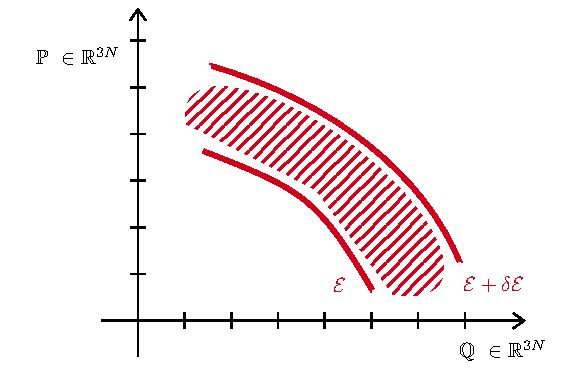
\includegraphics[width=0.5\textwidth]{\main/Images/12_03_20/1.pdf}
    \caption{ Energy shell between $\mathcal{E}$ and $\mathcal{E}+\delta \mathcal{E}$ in the microcanonical ensamble\label{fig:energy-shell}.}
\end{figure}

\medskip

The energy associated with a certain microstate is given by the \textbf{Hamiltonian}  function:
\begin{align}\label{eqn:hamiltonian}
    H(\mathbb{Q},\mathbb{P}) = \sum_{i=1}^N \frac{\norm{\bm{p_i}}^2}{2m_i} + U(\mathbb{\mathbb{Q}}) 
\end{align}
where $U(\mathbb{Q})$ is the potential energy associated with the (conservative) forces $\bm{F_i}$:
\begin{align*}
    \bm{F_i}(\mathbb{Q}) = - \grad_{\bm{r_i}} U = \left(-\pdv{U}{x_i}, - \pdv{U}{y_i}, -\pdv{U}{z_i}\right)^T
\end{align*}
We can rewrite Newton's equations (\ref{eqn:equations}) by using the Hamiltonian as follows:
\begin{align*}
    \dot{q}_\alpha &=  \pdv{H(\mathbb{Q},\mathbb{P})}{p_\alpha} && q_\alpha \in \{x_i, y_i, z_i \colon i=1, \dots, N\}\\
    \dot{p}_\alpha &= -\pdv{H(\mathbb{Q},\mathbb{P})}{q_\alpha}
    && p_\alpha \in \{p_{xi}, p_{yi}, p_{zi} \colon i = 1, \dots, N\}
\end{align*}

So the energy shell $D$ between $\mathcal{E}$ and $\mathcal{E}+ \delta \mathcal{E}$ can be written as:
\begin{align*}
    D \equiv \{(\mathbb{Q},\mathbb{P}) \colon \mathcal{E} \leq H(\mathbb{Q}, \mathbb{P}) < \mathcal{E}+ \delta \mathcal{E}\} \subset \mathbb{R}^{6N}
\end{align*}
Then, as consequence of $\mathcal{H}$, we construct a uniform distribution over $D$:
\begin{align}\label{eqn:pQP}
    \mathcal{P}(\mathbb{Q},\mathbb{P}) &= \frac{1}{\mathcal{Z}} [\theta(\mathcal{E}+ \delta \mathcal{E} - H(\mathbb{Q},\mathbb{P})) - \theta(\mathcal{E}-H(\mathbb{Q},\mathbb{P}))] =\\
    &= \begin{cases} 
        \frac{1}{\mathcal{Z}} & \mathcal{H}\in [\mathcal{E}, \mathcal{E}+\delta \mathcal{E}]\\
        0 & \text{otherwise} 
    \end{cases} \nonumber
\end{align}
where $\mathcal{Z}$ is just the normalization constant:
\begin{align}\label{eqn:Z-def}
    \mathcal{Z} = \int_{\mathbb{R}^{6N}} \underbrace{\dd[3N]{\bm{q}}\dd[3N]{\bm{p}}}_{\dd{\bm{\Gamma}}}\> [\theta(\mathcal{E}+\delta \mathcal{E-H}) - \theta(\mathcal{E}-H)]
\end{align}
where $H\equiv H(\mathbb{Q},\mathbb{P})$ for brevity.

\medskip

We then expand the difference of $\theta$ functions to first order:
\begin{align} \label{eqn:heav-deriv}
    \theta(\mathcal{E}+\delta \mathcal{E}-H) - \theta(\mathcal{E}-H) = \delta \mathcal{E} \pdv{\mathcal{E}} \theta(\mathcal{E}-H) \approx \delta \mathcal{E}\, \delta(\mathcal{E}-H)
\end{align} 
where we used the \textit{distributional derivative} for the Heaviside function, which is the Dirac delta $\delta$. %Insert remainder to chap 2 of Baiesi notes 

We neglect all higher orders in $\delta\mathcal{E}$, as, as we will then send $\delta \mathcal{E} \to 0$.

\medskip

Substituting (\ref{eqn:heav-deriv}) in (\ref{eqn:Z-def}) we get:
\begin{align}\label{eqn:z-omega}
    \mathcal{Z}= \int_{\mathbb{R}^{6N}} \dd{\bm{\Gamma}} \delta(\mathcal{E}-H)\delta \mathcal{E} \equiv \Omega(\mathcal{E}) \delta \mathcal{E}
\end{align}
where we defined:
\begin{align}\label{eqn:omega-def}
    \Omega(\mathcal{E}) = \int_{\mathbb{R}^{6N}} \dd{\bm{\Gamma}} \delta(\mathcal{E}-H(\mathbb{Q},\mathbb{P}))
\end{align}

\begin{comment}
In order to prove the $\mathcal{H}$ hypothesis one should show that that the trajectories solving the equations of motion \textit{visit} \q{equally} all possible states. This cannot be done in the interesting cases, and so we can just derive consequences from $\mathcal{H}$ and compare them to experiments.

Note that every point in phase-space represents \textit{full information} about the system - i.e. the positions and momenta of all the particles.
\end{comment}

\end{document}
